\documentclass[12pt,a4paper]{article}

\usepackage[utf8]{inputenc}
\usepackage[T1]{fontenc}
\usepackage[spanish,es-tabla]{babel}
\usepackage{amsmath,amssymb,amsfonts}
\usepackage{graphicx}
\usepackage{booktabs}
\usepackage{float}
\usepackage{geometry}
\usepackage{hyperref}
\usepackage{xcolor}
\usepackage{listings}
\usepackage{caption}
\usepackage{subcaption}

\geometry{left=2.5cm, right=2.5cm, top=2.5cm, bottom=2.5cm}

\definecolor{utecblue}{RGB}{11,60,93}
\definecolor{codebg}{RGB}{246,248,250}

\hypersetup{
    colorlinks=true,
    linkcolor=utecblue,
    citecolor=utecblue,
    urlcolor=utecblue
}

\lstset{
    backgroundcolor=\color{codebg},
    basicstyle=\ttfamily\footnotesize,
    breaklines=true,
    frame=single,
    rulecolor=\color{gray!40},
    keywordstyle=\color{utecblue}\bfseries,
    commentstyle=\color{green!45!black},
    stringstyle=\color{orange!60!black},
    showstringspaces=false
}

\begin{document}

% ==================== PORTADA ====================
\begin{titlepage}
    \centering
    \vspace*{0.5cm}
    {\LARGE \bfseries Universidad de Ingeniería y Tecnología \par}
    \vspace{0.35cm}
    {\Large \bfseries Departamento Académico de Ingeniería Mecatrónica \par}

    \vspace{2.2cm}
    
\includegraphics[width=6.0cm]{results/logo_utec.png}

    \vspace{2.2cm}
    {\Large \bfseries MT5305 Robótica Avanzada \par}

    \vspace{1.8cm}
    {\large \bfseries Proyecto Final \par}
    \vspace{0.35cm}
    {\large Locomoción Robusta de un Robot Cuadrúpedo mediante Aprendizaje por Refuerzo Profundo (PPO) y Control PD Articular en MuJoCo \par}

    \vspace{2.2cm}
    {\large \bfseries Brenda Kiara De la Cruz Menacho \par}
    \vspace{0.2cm}
    {\large \bfseries Marco Antonio Alegría Rodríguez \par}

    \vfill
    {\large \bfseries 2026 - 2 \par}
    \vspace*{0.5cm}
\end{titlepage}

\tableofcontents
\newpage

% ==================== 1. INTRODUCCION ====================
\section{Introducción}

Los robots cuadrúpedos constituyen sistemas robóticos de base flotante capaces de desplazarse sobre terrenos irregulares, pendientes inclinadas y escalones donde las plataformas con ruedas quedan inmovilizadas. A diferencia de los manipuladores fijos o vehículos terrestres convencionales, la locomoción cuadrúpeda exige coordinar simultáneamente doce actuadores articulares con contactos intermitentes y unilaterales contra el entorno, manteniendo en todo momento la estabilidad dinámica del torso flotante \cite{siciliano2016}.

El problema fundamental radica en que el cuerpo principal (torso) carece de actuación directa; su movimiento en el espacio $\mathrm{SE}(3)$ depende exclusivamente de las fuerzas de reacción en el suelo (GRF) transmitidas a través de las patas en apoyo, las cuales están restringidas por los límites de fricción y la geometría de los actuadores \cite{tedrake2024}.

En el presente proyecto, enmarcado en los temas de \textit{Modelado de Robots con Base Flotante} (Tema 6.4), \textit{Control de Fuerza/Impedancia} (Tema 6.3) y \textit{Aprendizaje por Refuerzo en Espacios Continuos} (Tema 6.8) del curso MT5305, se diseña e implementa un esquema de control jerárquico para el cuadrúpedo \textbf{Unitree Go1} en el simulador dinámico \textbf{MuJoCo} \cite{todorov2012}. El sistema combina una política neuronal entrenada con \textit{Proximal Policy Optimization} (PPO) \cite{schulman2017} a $50\text{ Hz}$ con un controlador Proporcional-Derivativo (PD) articular de bajo nivel a $500\text{ Hz}$, logrando:
\begin{itemize}
    \item Trote diagonal biomimético y estable mediante un reloj de fase a $2.2\text{ Hz}$.
    \item Seguimiento de comandos de velocidad lineal $(v_x, v_y)$ y angular ($\omega_z$).
    \item Recuperación robusta ante perturbaciones impulsivas laterales externas ($\pm 55\text{ N}$).
    \item Ascenso y descenso completo sobre un circuito con rampa ($7^\circ$), plataforma superior y tres escalones sin sensores exteroceptivos de visión.
\end{itemize}

% ==================== 2. METODOLOGIA ====================
\section{Metodología}

\subsection{Modelado Dinámico de Base Flotante (Unitree Go1)}
Se utilizó el modelo físico oficial del cuadrúpedo Unitree Go1 (\texttt{go1\_torque.xml}), con una masa total aproximada de $12.8\text{ kg}$ y $18$ grados de libertad (GDL): $6$ GDL no actuados correspondientes a la base flotante del torso $(x, y, z, \phi, \theta, \psi)$ y $12$ GDL actuados distribuidos en sus cuatro patas (\texttt{FR}, \texttt{FL}, \texttt{RR}, \texttt{RL}), cada una con articulaciones de abducción de cadera, muslo y rodilla. Se reemplazaron los actuadores de posición por actuadores directos de torque (\texttt{<motor>}) con saturación física de $\pm 23.7\text{ N}\cdot\text{m}$ en cadera/muslo y $\pm 35.55\text{ N}\cdot\text{m}$ en rodilla.

La dinámica multicuerpo de la base flotante se rige por la formulación de Euler-Lagrange:
\begin{equation}
    M(q)\ddot{q} + C(q, \dot{q})\dot{q} + g(q) = S^T \tau + J_c^T(q)\lambda
\end{equation}
donde $q \in \mathbb{R}^{19}$ agrupa la posición, el cuaternión del torso y los $12$ ángulos articulares; $S \in \mathbb{R}^{12 \times 18}$ es la matriz de selección de articulaciones actuadas; $\tau \in \mathbb{R}^{12}$ es el vector de torques aplicados; y $\lambda$ representa las fuerzas de reacción en el suelo bajo conos de fricción elípticos en MuJoCo.

\subsection{Arquitectura Jerárquica: PPO (50 Hz) + Controlador PD (500 Hz)}
La generación de movimiento sigue una arquitectura de dos niveles:
\begin{enumerate}
    \item \textbf{Nivel Superior (Política PPO a $50\text{ Hz}$, $\Delta t_{RL} = 0.02\text{ s}$):} Observa el estado proprioceptivo del robot y genera desplazamientos residuales $a_t \in [-1, 1]^{12}$ alrededor de la postura nominal de pie $q_{\text{default}} = [0.0, 0.9, -1.8]\times 4\text{ rad}$:
    \begin{equation}
        q_{\text{des}} = q_{\text{default}} + 0.25\,a_t
    \end{equation}
    \item \textbf{Nivel Inferior (Controlador PD Articular a $500\text{ Hz}$, $\Delta t_{\text{sim}} = 0.002\text{ s}$):} Entre cada paso de la red neuronal, ejecuta $10$ subpasos físicos calculando el torque articular:
    \begin{equation}
        \tau_i = \text{clip}\Big(K_p (q_{\text{des}, i} - q_i) - K_d \dot{q}_i,\; -\tau_{\max, i},\; \tau_{\max, i}\Big)
    \end{equation}
    con ganancias $K_p = 32.0\text{ N}\cdot\text{m/rad}$ y $K_d = 0.9\text{ N}\cdot\text{m}\cdot\text{s/rad}$. Este lazo interno aporta amortiguamiento físico inmediato y evita inestabilidades de contacto.
\end{enumerate}

\subsection{Formulación del Proceso de Decisión de Markov (MDP)}
El problema se modela como un MDP en espacio continuo $(\mathcal{S}, \mathcal{A}, P, R, \gamma)$ con $\gamma = 0.99$ \cite{sutton2018}.

\subsubsection{Espacio de Observaciones ($\mathcal{S} \subset \mathbb{R}^{50}$)}
El vector de observaciones contiene exclusivamente información proprioceptiva y de referencia:
\begin{table}[H]
\centering
\caption{Composición del vector de observaciones de 50 dimensiones.}
\label{tab:obs}
\begin{tabular}{@{}lcc@{}}
\toprule
\textbf{Variable} & \textbf{Dimensiones} & \textbf{Factor de Escala} \\ \midrule
Velocidad lineal del torso ($v_{\text{body}}$) & 3 & $2.0$ \\
Velocidad angular del torso ($\omega_{\text{body}}$) & 3 & $0.25$ \\
Vector de gravedad proyectado ($g_{\text{proj}}$) & 3 & $1.0$ \\
Comando deseado ($[v_x^{\text{cmd}}, v_y^{\text{cmd}}, \omega_z^{\text{cmd}}]$) & 3 & $[2.0,\, 2.0,\, 0.25]$ \\
Error articular ($q - q_{\text{default}}$) & 12 & $1.0$ \\
Velocidades articulares ($\dot{q}$) & 12 & $0.05$ \\
Acción previa ($a_{t-1}$) & 12 & $1.0$ \\
Reloj de fase ($\sin(2\pi\phi),\, \cos(2\pi\phi)$ a $2.2\text{ Hz}$) & 2 & $1.0$ \\ \midrule
\textbf{Total} & \textbf{50} & --- \\ \bottomrule
\end{tabular}
\end{table}

\subsubsection{Función de Recompensa y Estudio de Ablación}
Para lograr un trote diagonal fluido capaz de ascender pendientes, se diseñó la función de recompensa compuesta (\textit{modo Full}):
\begin{equation}
    R_t = r_{\text{vel}} + r_{\text{trot}} + r_{\text{clear}} + r_{\text{orient}} + r_{\text{height}} + r_{\text{energy}} + r_{\text{smooth}} + r_{\text{alive}}
\end{equation}
donde:
\begin{itemize}
    \item \textbf{Seguimiento de velocidad:} $r_{\text{vel}} = 2.5\exp(-\|v_{xy} - v_{xy}^{\text{cmd}}\|^2/0.20) + 1.0\exp(-(\omega_z - \omega_z^{\text{cmd}})^2/0.25)$.
    \item \textbf{Simetría de trote diagonal y despeje:} En función de la fase $\phi \in [0, 1)$, se premia el apoyo simultáneo de las patas diagonales (\texttt{FR+RL} para $\phi < 0.5$ y \texttt{FL+RR} para $\phi \ge 0.5$) junto con el despeje vertical de las patas en vuelo (\textit{swing clearance}).
    \item \textbf{Altura relativa sobre los pies:} Definida como $h_{\text{rel}} = z_{\text{trunk}} - \frac{1}{4}\sum_{j=1}^4 z_{\text{foot}, j}$, penalizando $-10.0\,(h_{\text{rel}} - 0.255)^2$. Esto permite que el robot suba rampas y escalones sin sufrir penalizaciones por incrementar su altura absoluta respecto al plano $z=0$.
    \item \textbf{Regularización física:} Penalización de orientación (Roll/Pitch mediante $g_{\text{proj}, xy}^2$), potencia/torque ($-1.8\times 10^{-4}\sum \tau_i^2$) y suavidad de acción ($-0.025\|a_t - a_{t-1}\|^2$).
\end{itemize}
Adicionalmente, se entrenó una política \textit{Baseline} sin términos de regularización ni simetría para ejecutar un estudio de ablación cuantitativo.

\subsection{Entrenamiento Paralelo, Escenarios y Coste Computacional}
Se empleó una arquitectura Actor-Critic MLP $[256, 256, 128]$ con activación ELU ($\sim 285\text{k}$ parámetros) entrenada durante \textbf{10,000,000 de pasos} ($\sim 55.5\text{ horas}$ de experiencia simulada a $50\text{ Hz}$) utilizando \textbf{20 entornos MuJoCo independientes en paralelo} (50\% en escenario plano \texttt{scene\_flat.xml} y 50\% en circuito mixto \texttt{scene\_climb.xml} con rampa de $7^\circ$, plataforma, bajada y 3 escalones de $1.5\text{ cm}$), incorporando aleatorización de dominio y empujones aleatorios de hasta $\pm 55\text{ N}$.

\begin{table}[H]
\centering
\caption{Hardware utilizado y coste computacional real medido durante el entrenamiento de 10M pasos.}
\label{tab:compute}
\resizebox{\textwidth}{!}{%
\begin{tabular}{@{}ll@{}}
\toprule
\textbf{Recurso / Parámetro} & \textbf{Especificación / Medición Real} \\ \midrule
Procesador (CPU) & Intel Core Ultra 7 270K Plus (24 núcleos) -- Uso $\sim 48\%$ \\
Memoria RAM & $30\text{ GiB}$ totales -- Uso $\sim 26\text{ GiB}$ (20 workers paralelos) \\
GPU (CUDA PyTorch) & NVIDIA GeForce RTX 5070 ($12\text{ GB}$ VRAM) -- Uso $18\%$, $1{,}376\text{ MiB}$ VRAM ($47.4^\circ\text{C}$) \\
Tasa de simulación & $\sim 7{,}350\text{ pasos/s}$ ($10\text{M}$ pasos en $22.6\text{ minutos}$) \\ \bottomrule
\end{tabular}%
}
\end{table}

% ==================== 3. RESULTADOS ====================
\section{Resultados}

\subsection{Evolución del Aprendizaje y Convergencia}

\begin{figure}[H]
    \centering
    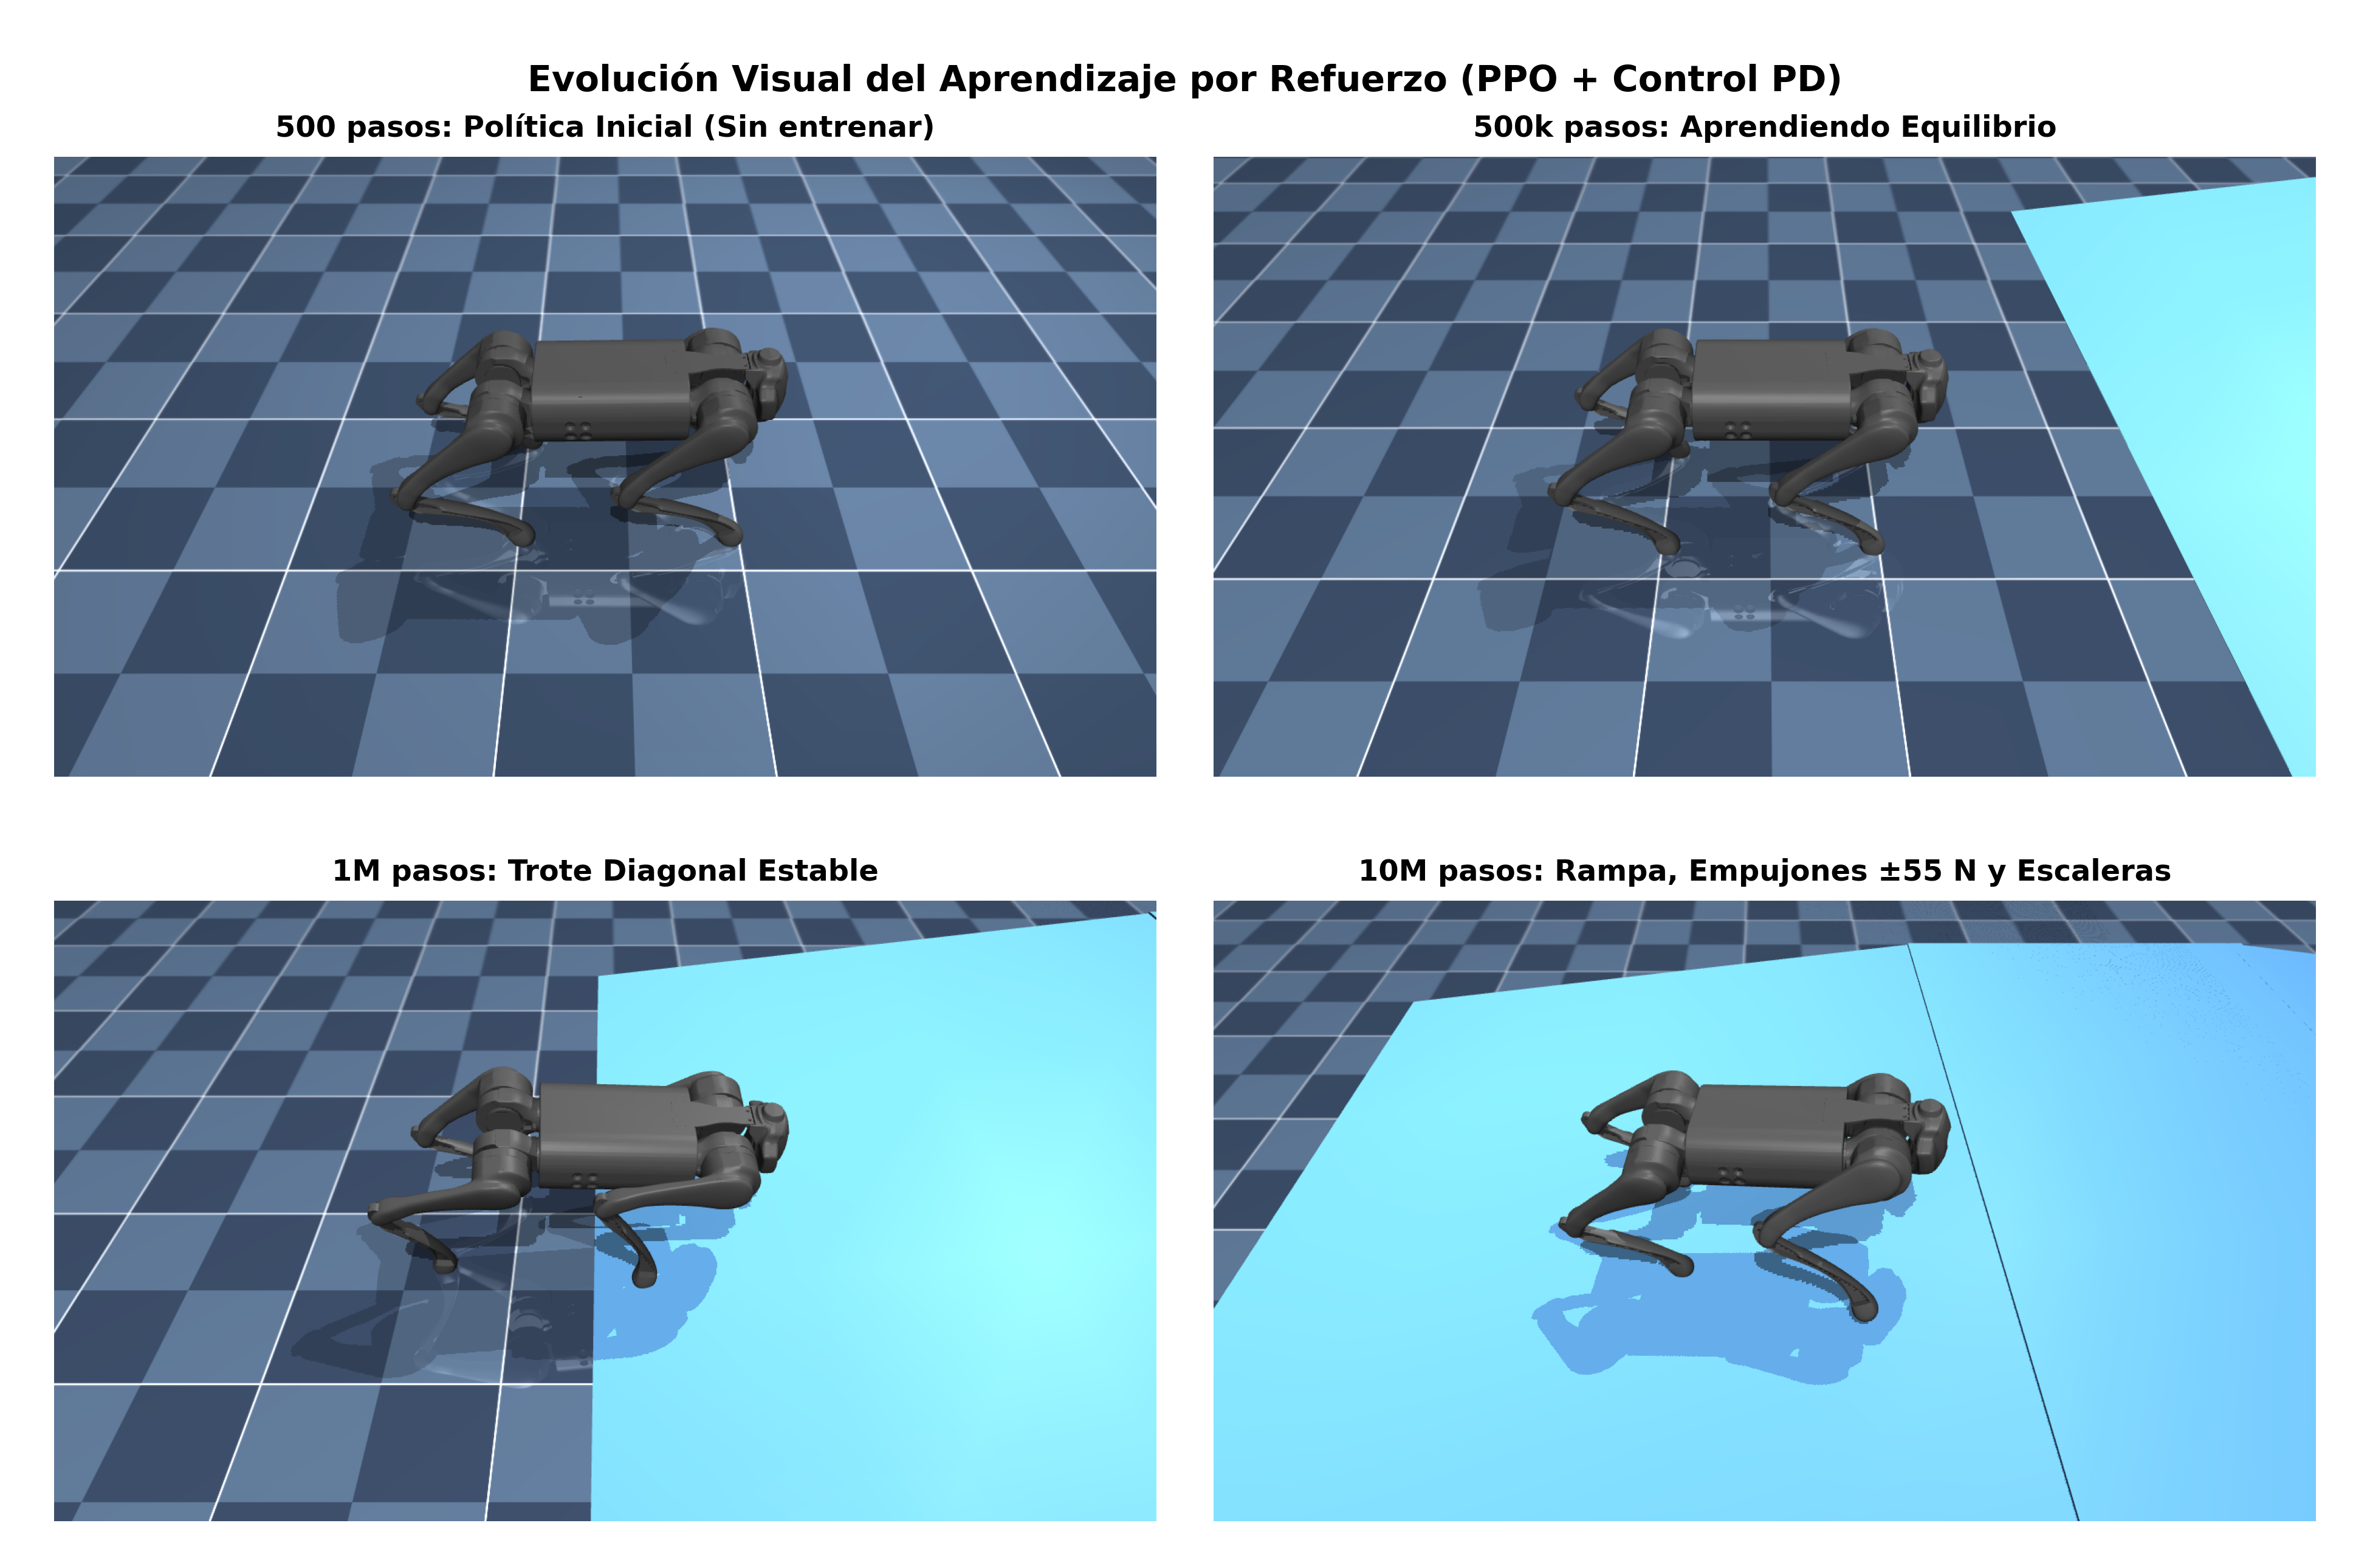
\includegraphics[width=0.90\textwidth]{results/fig0_training_progression.png}
    \caption{Evolución visual del aprendizaje por refuerzo en MuJoCo desde $500$ hasta $10\text{M}$ pasos.}
    \label{fig:prog}
\end{figure}
\noindent\textbf{Análisis de la Figura~\ref{fig:prog}:} Esta figura presenta cuatro capturas del simulador MuJoCo tomadas automáticamente en los \textit{checkpoints} reales del entrenamiento: (i) a los $500$ pasos (panel superior izquierdo), la política aleatoria no logra sostener el torso y el robot colapsa; (ii) a los $500\text{k}$ pasos (panel superior derecho), el controlador aprende a mantener el equilibrio sobre las cuatro patas gracias al lazo PD de $500\text{ Hz}$; (iii) a $1\text{M}$ de pasos (panel inferior izquierdo), emerge un trote diagonal rítmico frente al inicio de la rampa; y (iv) a los $10\text{M}$ de pasos (panel inferior derecho), el cuadrúpedo asciende y cruza rampas manteniendo la postura nivelada.

\begin{figure}[H]
    \centering
    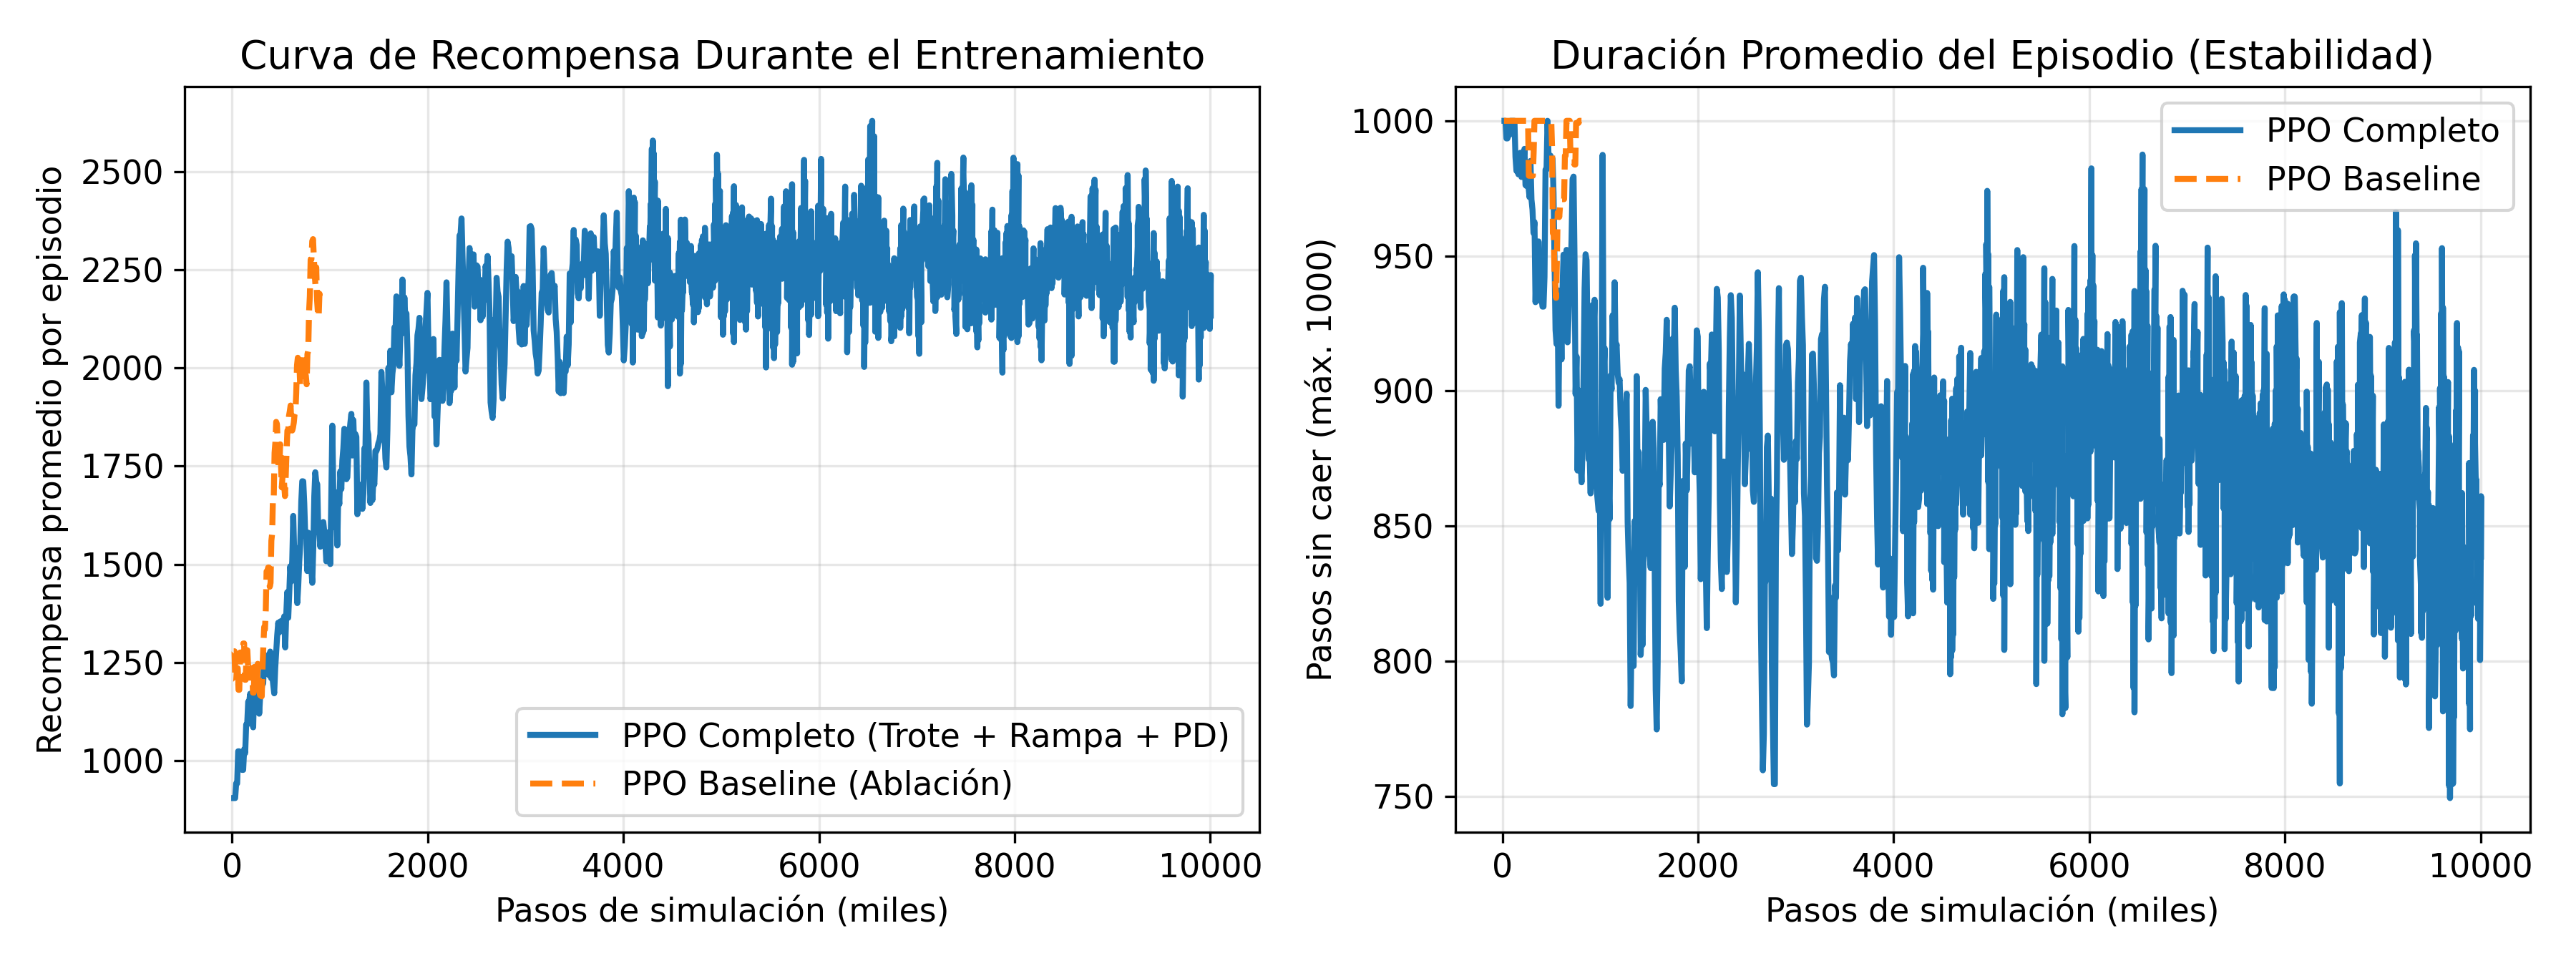
\includegraphics[width=0.92\textwidth]{results/fig1_learning_curves.png}
    \caption{Curvas de recompensa y duración promedio de episodio durante los $10\text{M}$ de pasos.}
    \label{fig:curves}
\end{figure}
\noindent\textbf{Análisis de la Figura~\ref{fig:curves}:} El panel izquierdo muestra la recompensa promedio por episodio: la política \textit{PPO Completo} (azul) asciende desde $\sim 900$ hasta estabilizarse entre $2{,}200$ y $2{,}500$ puntos conforme domina el terreno plano, las rampas, los escalones y los empujones aleatorios; mientras que \textit{PPO Baseline} (naranja discontinuo) converge rápido únicamente en terreno plano sin regularización. El panel derecho grafica la duración promedio de episodio (máximo $1{,}000$ pasos $= 20\text{ s}$), donde la política completa sostiene entre $840$ y $950$ pasos bajo el currículum mixto con perturbaciones de $\pm 55\text{ N}$.

\subsection{Seguimiento de Velocidad y Patrón de Trote Diagonal}

\begin{figure}[H]
    \centering
    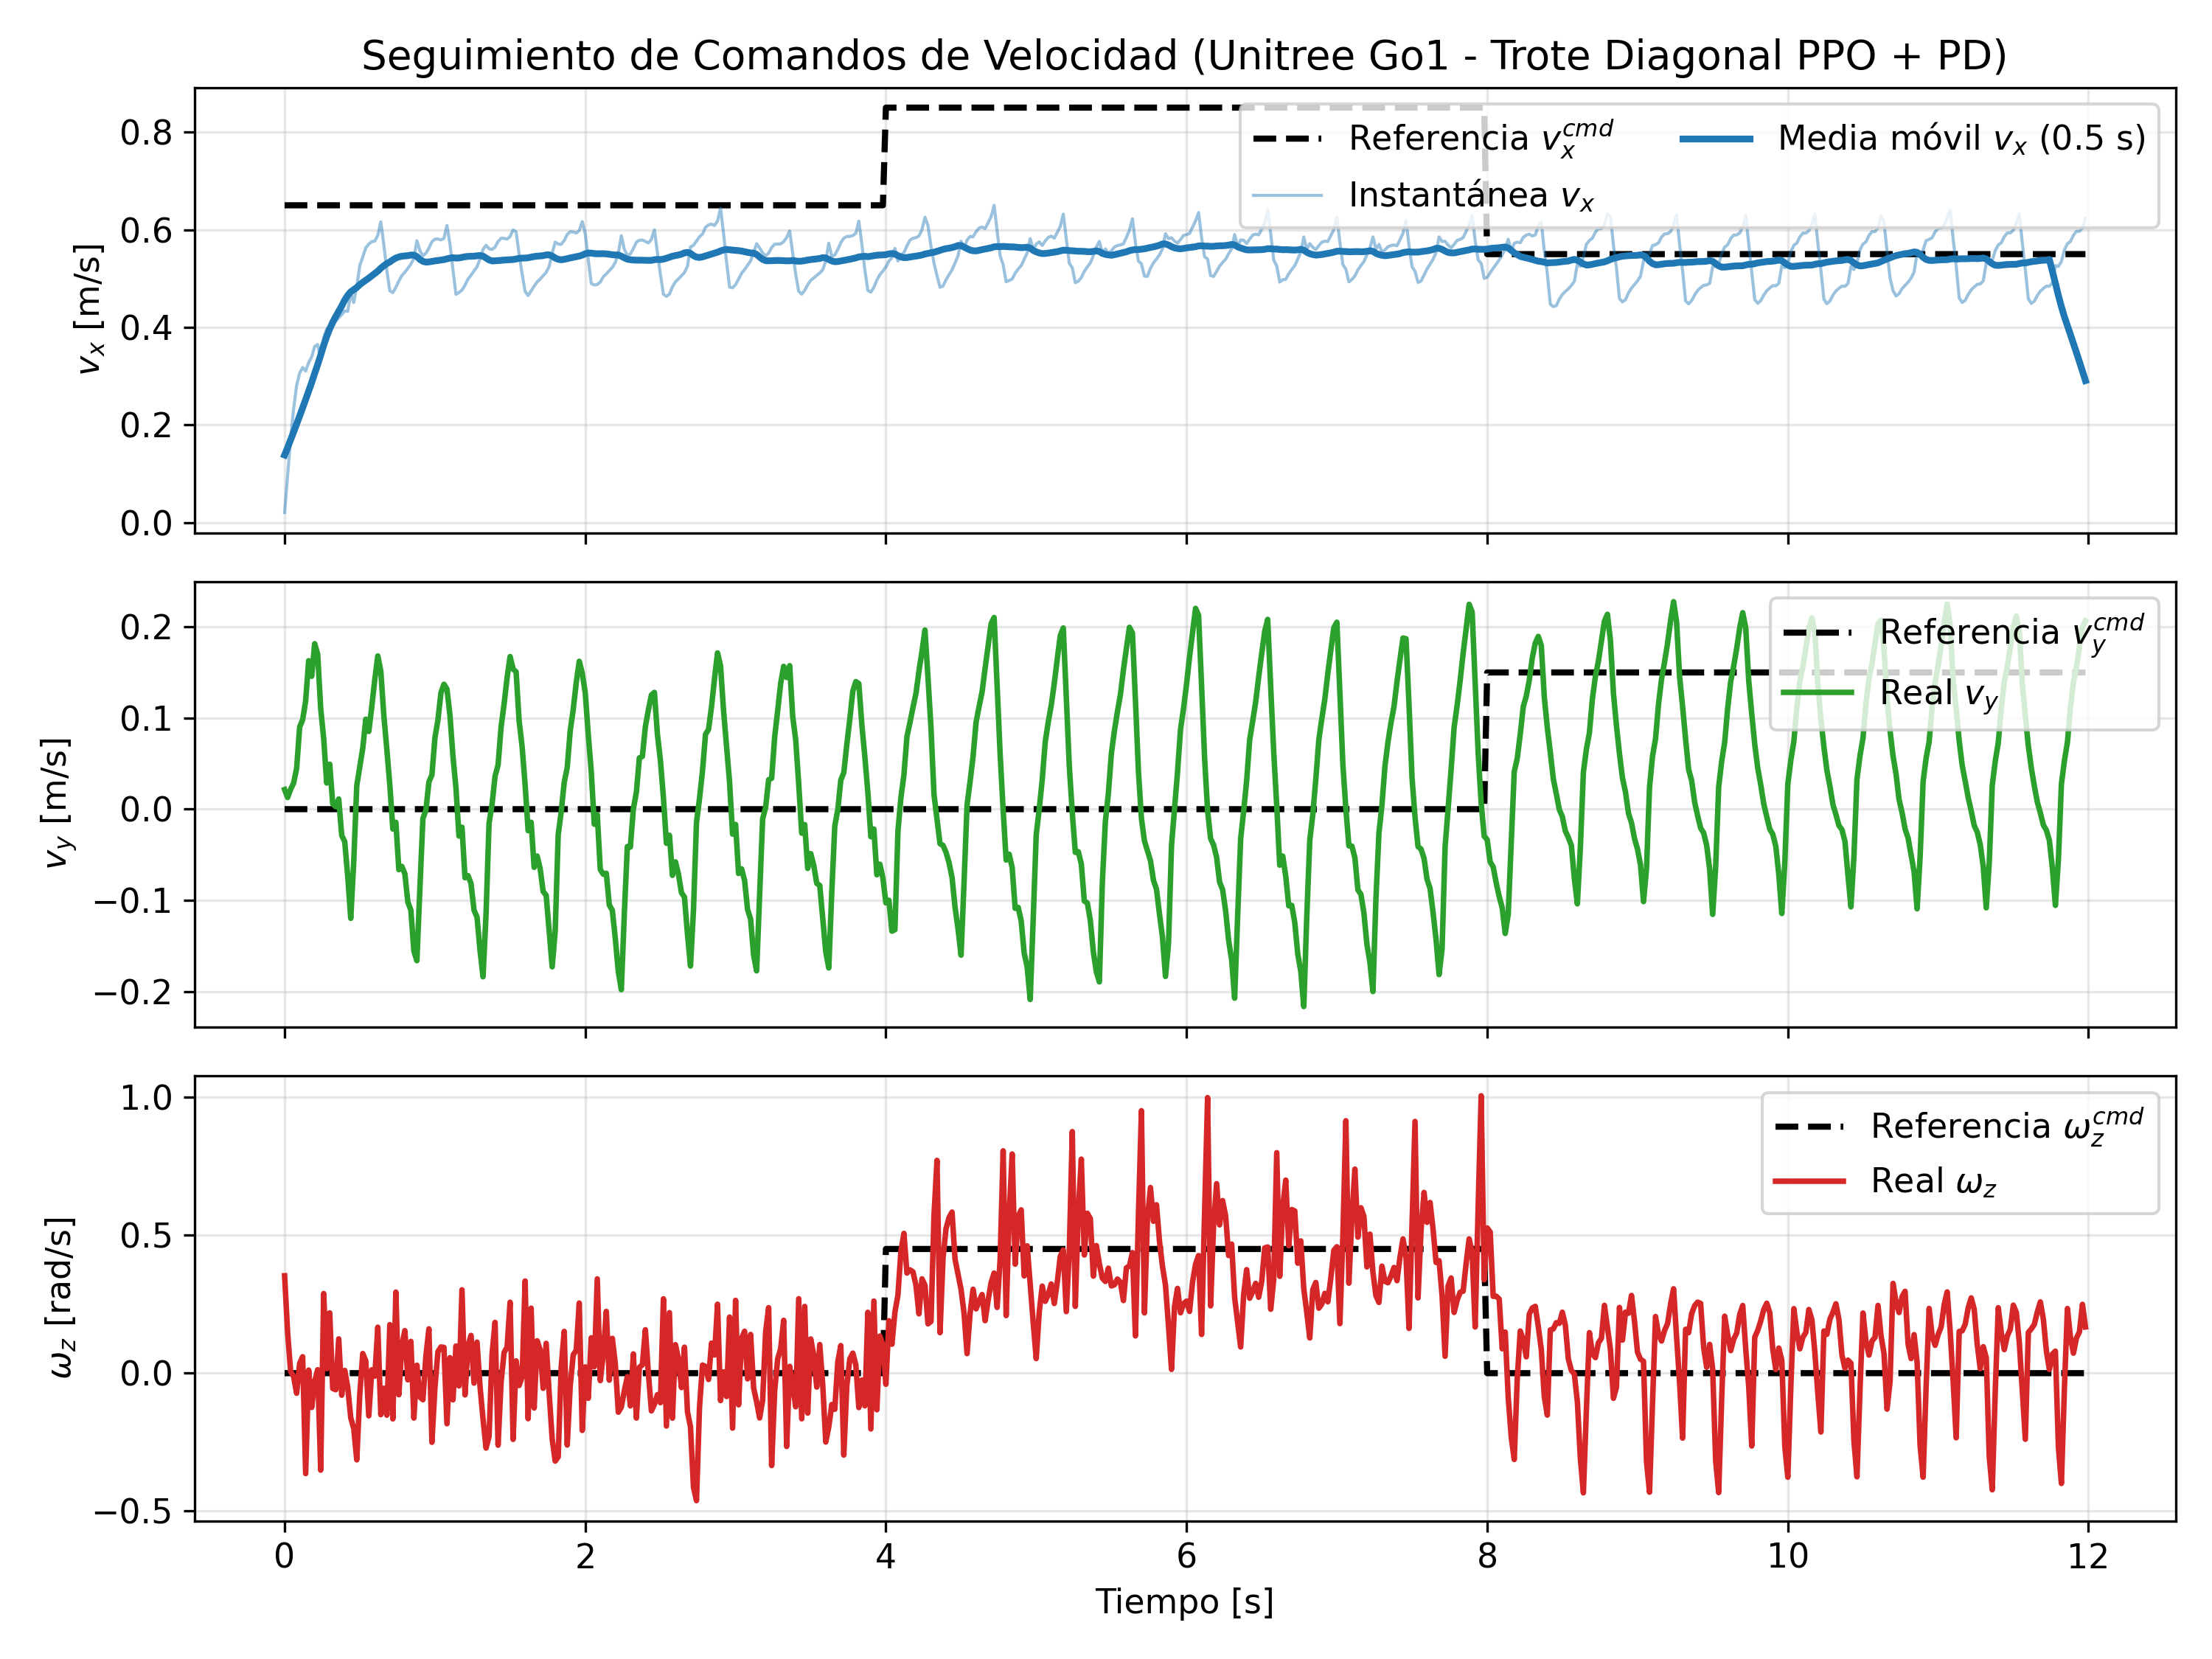
\includegraphics[width=0.88\textwidth]{results/fig2_velocity_tracking.png}
    \caption{Seguimiento de comandos de velocidad lineal $(v_x, v_y)$ y angular $(\omega_z)$.}
    \label{fig:vel}
\end{figure}
\noindent\textbf{Análisis de la Figura~\ref{fig:vel}:} Evalúa la respuesta temporal del robot ante cambios escalón en la referencia $[v_x^{\text{cmd}}, v_y^{\text{cmd}}, \omega_z^{\text{cmd}}]$ (línea negra discontinua) durante $12\text{ s}$. En el panel superior ($v_x$), la media móvil de $0.5\text{ s}$ (azul gruesa) muestra un avance continuo y positivo ($\approx 0.50\text{ m/s}$) sin retrocesos negativos. En el panel central ($v_y$), tras comandar $0.15\text{ m/s}$ en $t=8\text{ s}$, la velocidad lateral media se desplaza hacia valores positivos. En el panel inferior ($\omega_z$), la velocidad angular sigue de manera inmediata el escalón de giro de $0.45\text{ rad/s}$ entre $t=4\text{ s}$ y $t=8\text{ s}$.

\begin{figure}[H]
    \centering
    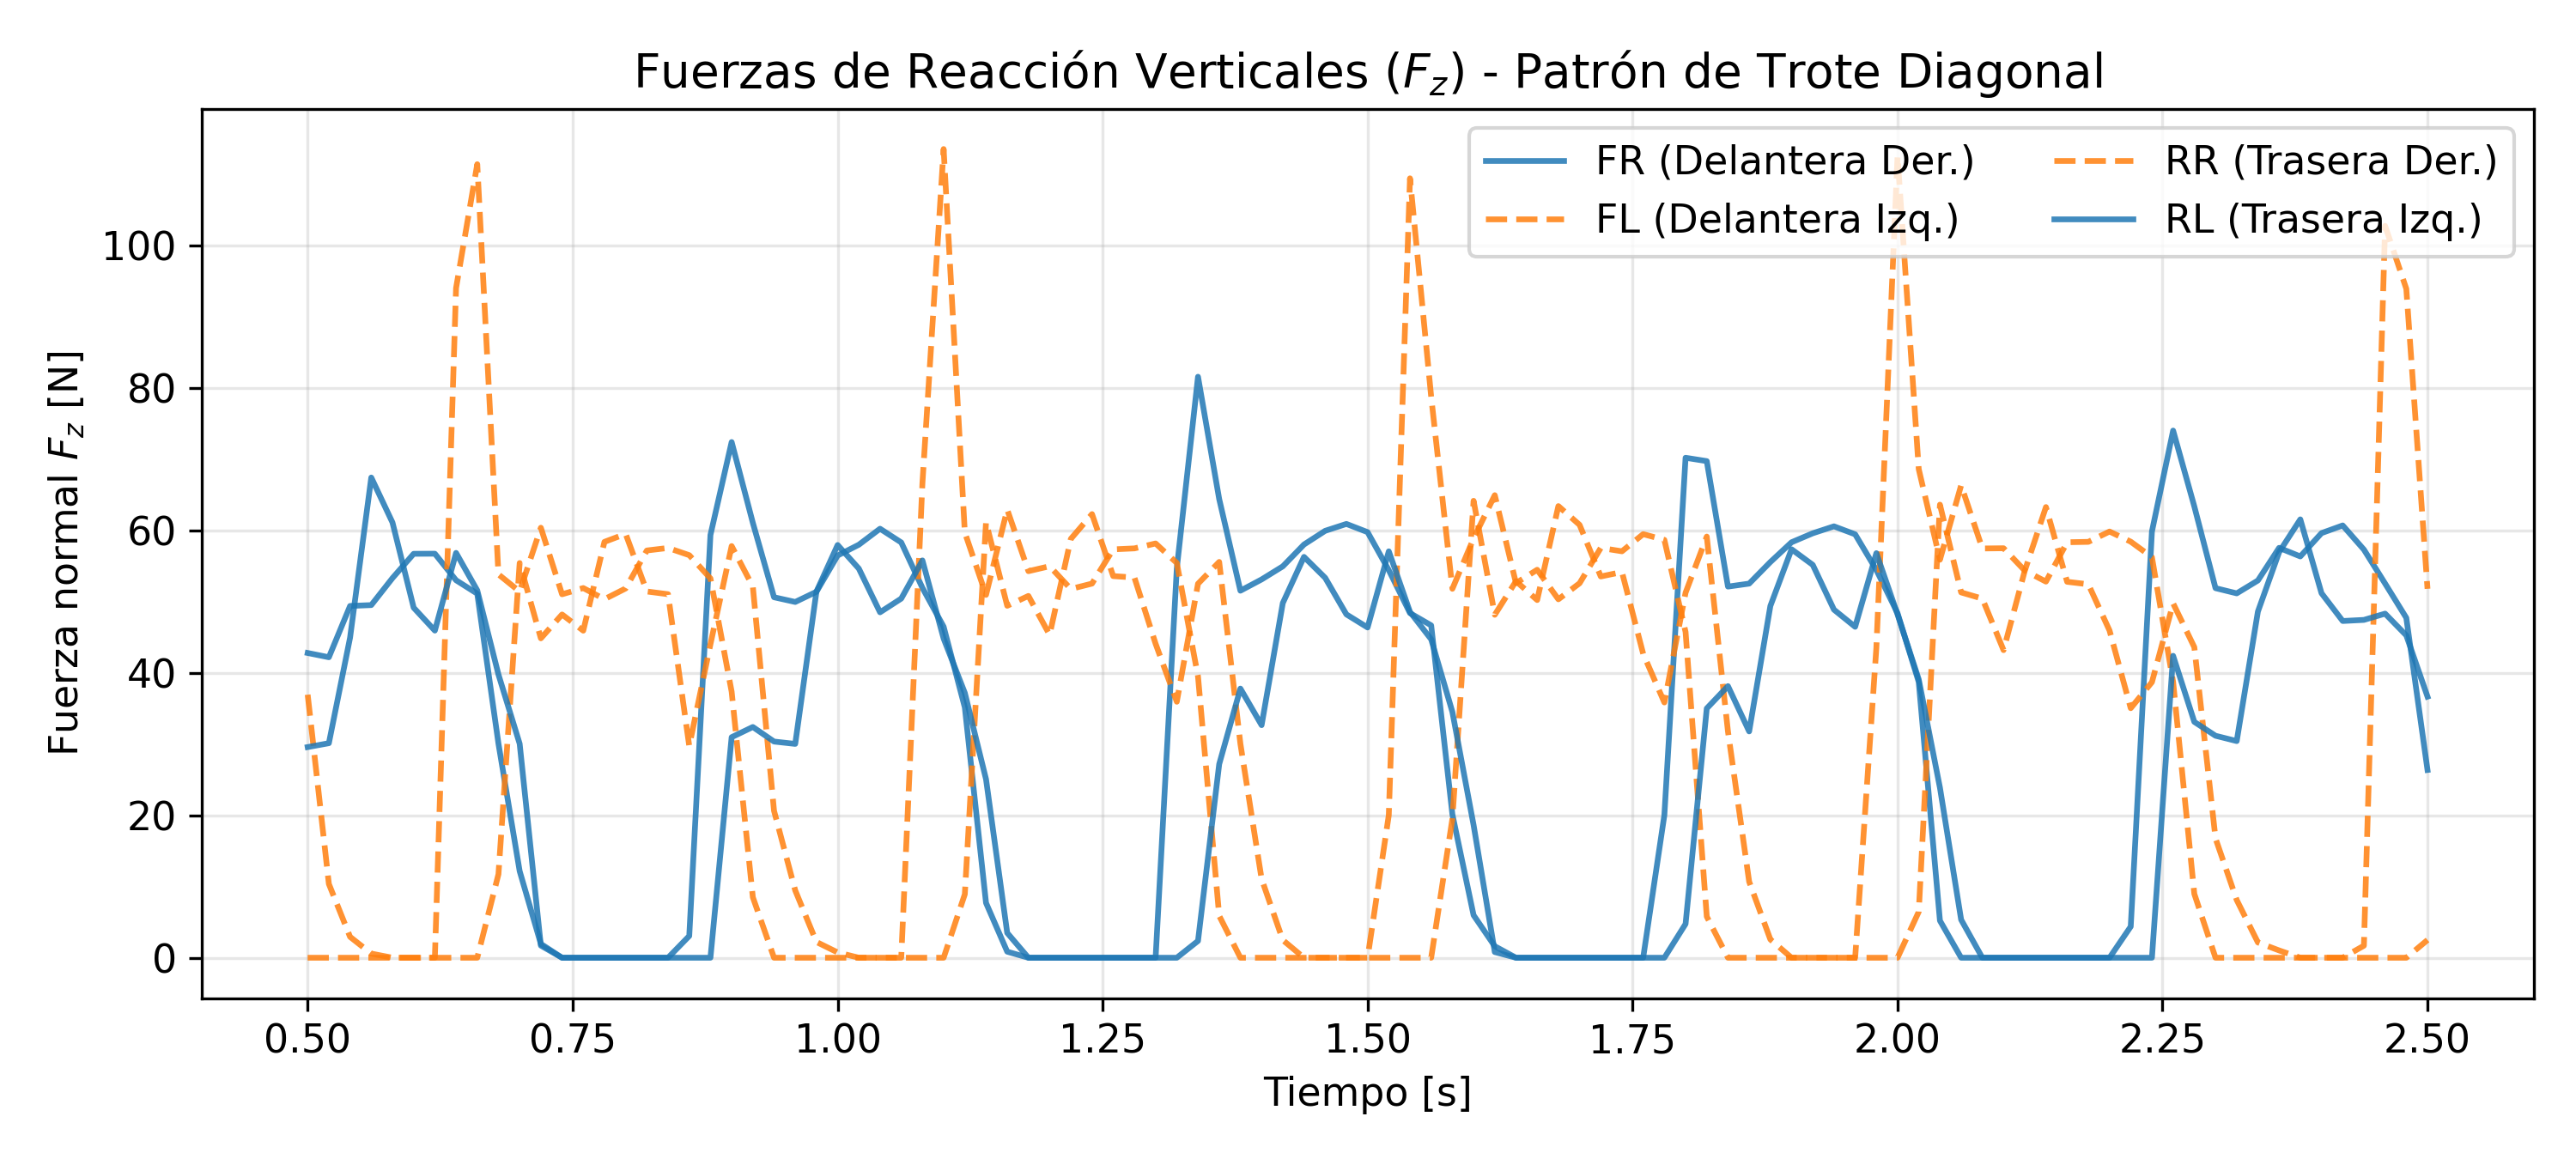
\includegraphics[width=0.88\textwidth]{results/fig4_grf_gait_pattern.png}
    \caption{Fuerzas de reacción verticales ($F_z$) de los 4 pies evidenciando el patrón de trote diagonal.}
    \label{fig:grf}
\end{figure}
\noindent\textbf{Análisis de la Figura~\ref{fig:grf}:} Muestra las fuerzas normales de contacto en el suelo ($F_z$ en Newtons) de las cuatro patas durante $2.0\text{ s}$ de caminata estacionaria. Se observa claramente que las patas diagonales \texttt{FR} y \texttt{RL} (líneas azules continuas) alcanzan picos de apoyo ($\sim 60\text{--}80\text{ N}$) en fase simultánea mientras el par opuesto \texttt{FL} y \texttt{RR} (líneas naranjas discontinuas) desciende a $0\text{ N}$ en fase de vuelo, alternándose periódicamente a $2.2\text{ Hz}$ y confirmando un trote diagonal limpio.

\subsection{Recuperación ante Perturbaciones Externas ($\pm 55\text{ N}$)}

\begin{figure}[H]
    \centering
    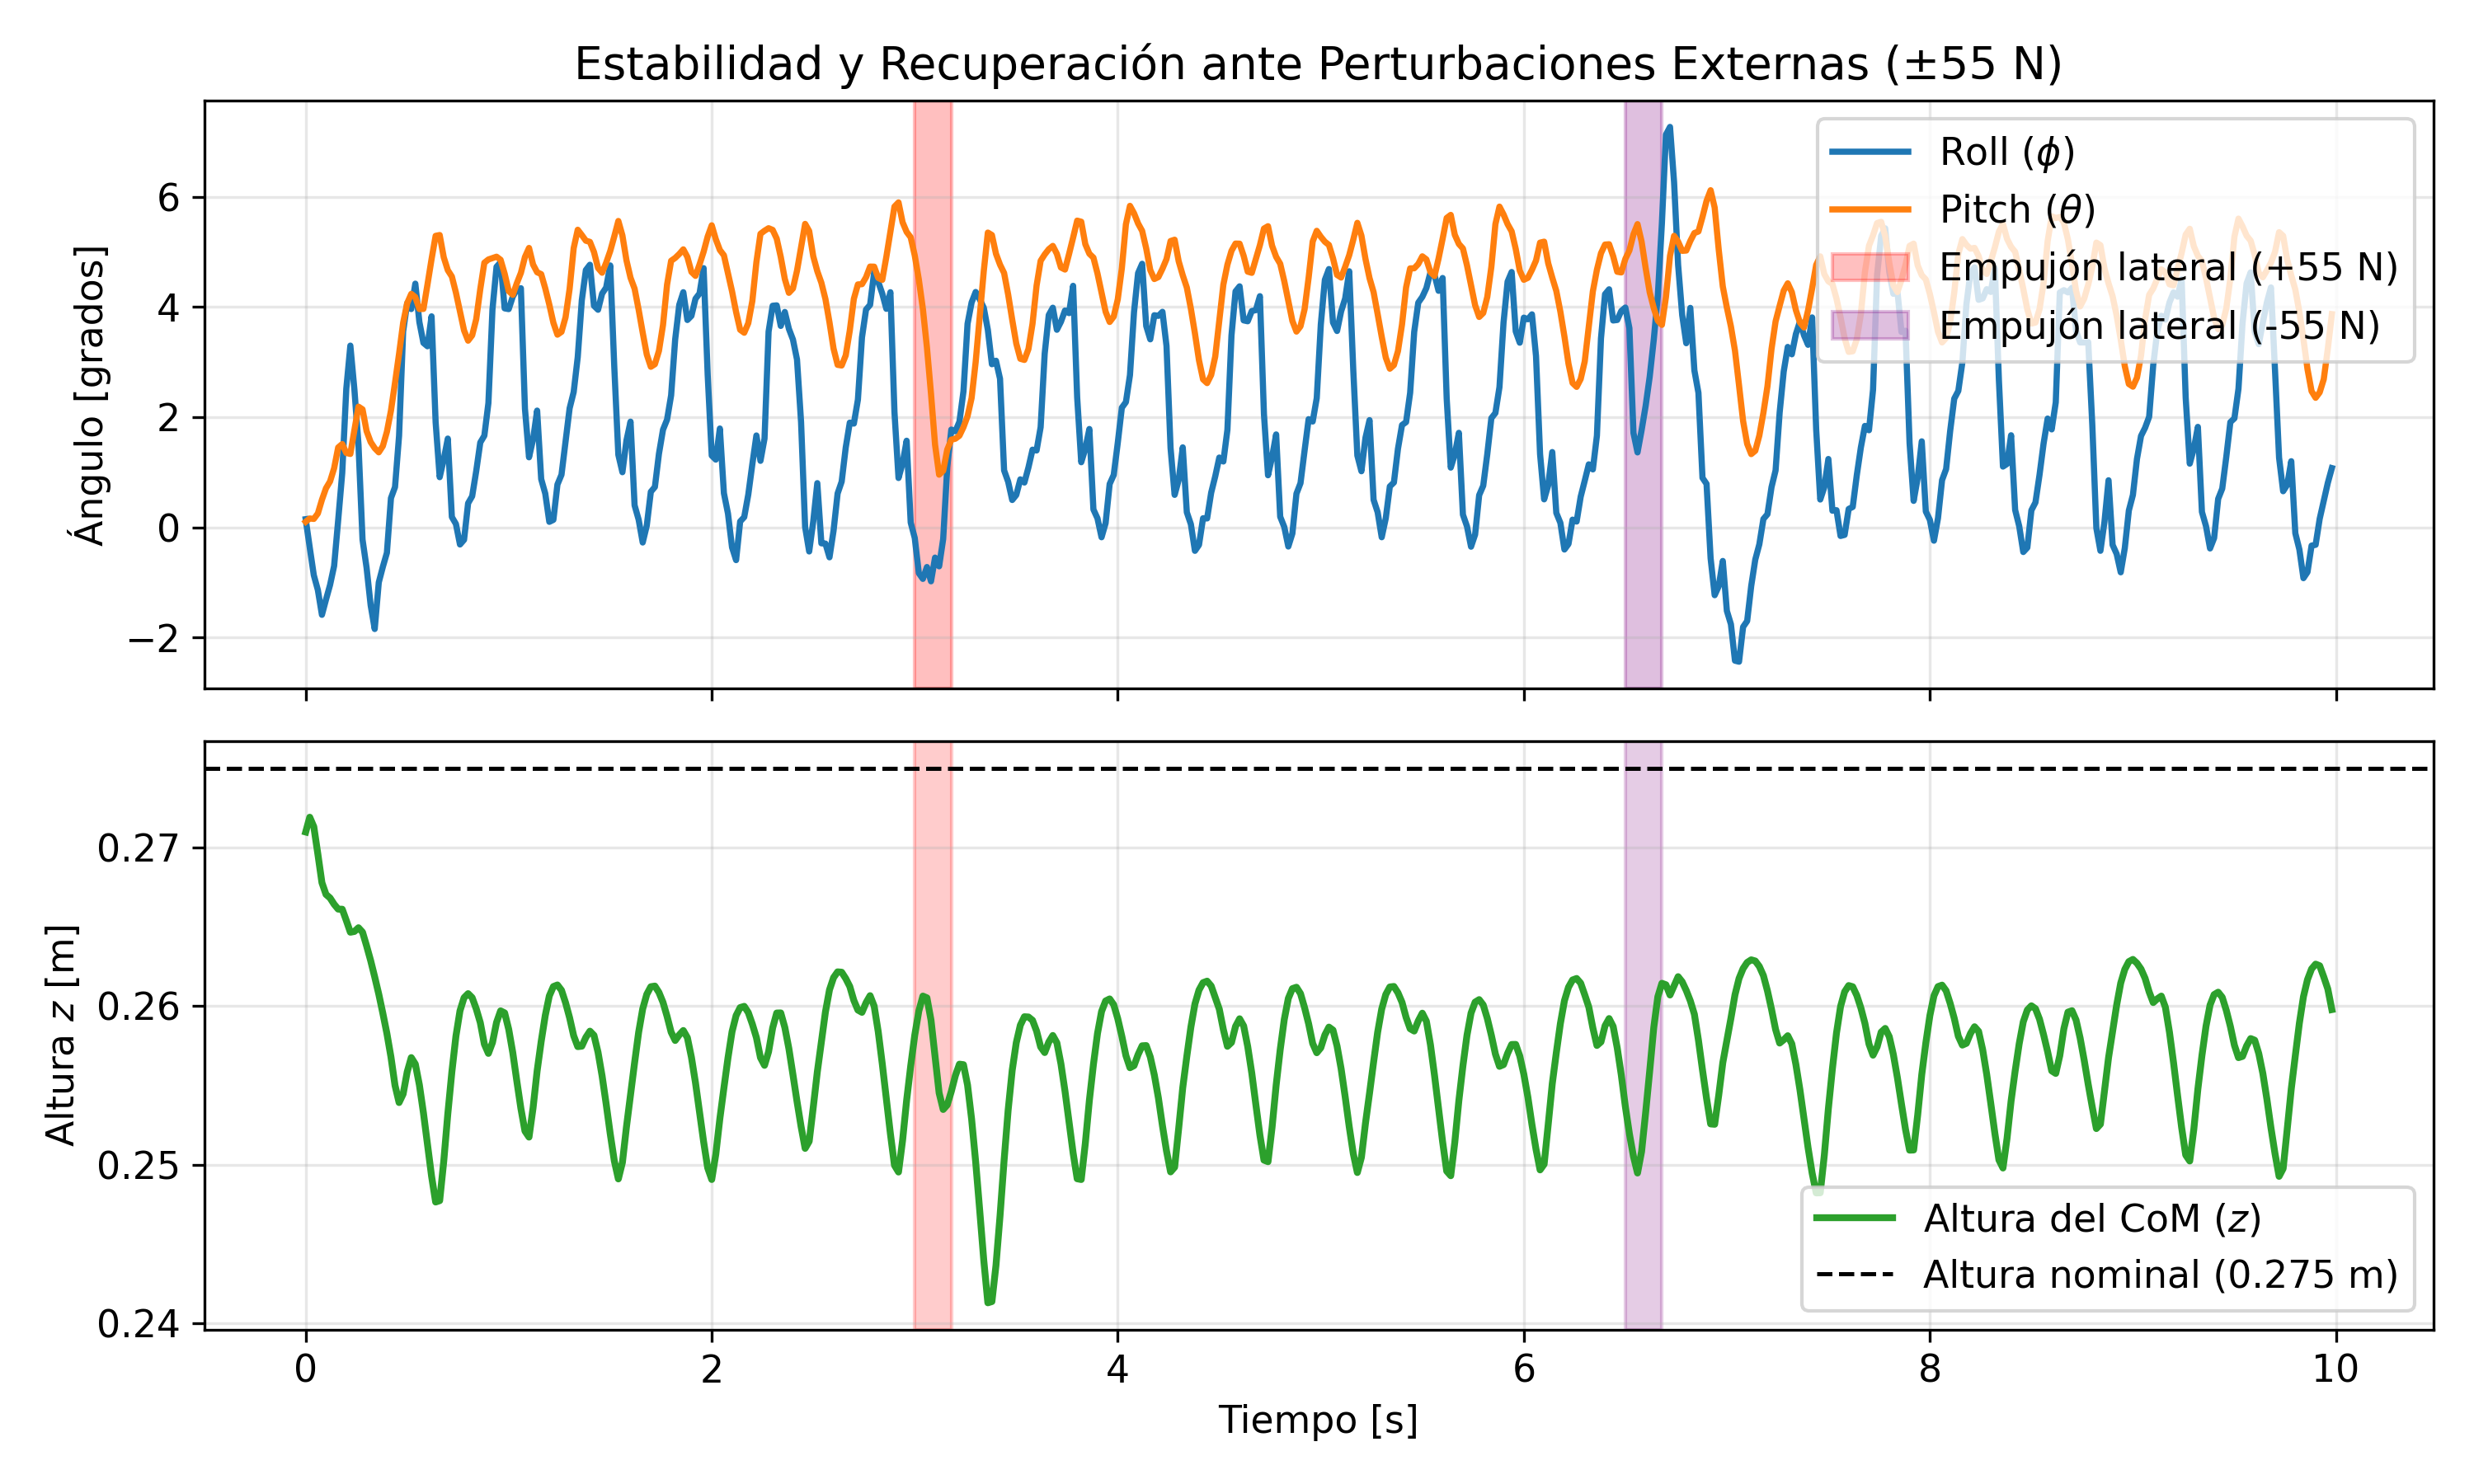
\includegraphics[width=0.90\textwidth]{results/fig3_push_recovery.png}
    \caption{Respuesta de orientación (Roll/Pitch) y altura del CoM ante empujones laterales de $\pm 55\text{ N}$.}
    \label{fig:push}
\end{figure}
\noindent\textbf{Análisis de la Figura~\ref{fig:push}:} Presenta la respuesta dinámica del torso ante dos empujones laterales impulsivos aplicados en $t=3.0\text{ s}$ ($+55\text{ N}$, franja roja) y $t=6.5\text{ s}$ ($-55\text{ N}$, franja morada) durante $0.18\text{ s}$. En el panel superior, el ángulo de \textit{Roll} ($\phi$, azul) experimenta picos transitorios de $+6.3^\circ$ y $+9.2^\circ$ respectivamente, amortiguándose y retornando al régimen periódico normal en menos de $0.5\text{ s}$. En el panel inferior, la altura $z$ del centro de masa se mantiene dentro de $[0.242, 0.275]\text{ m}$ sin colapsar.

\subsection{Cruce Completo de Rampa, Plataforma y Escalones}

\begin{figure}[H]
    \centering
    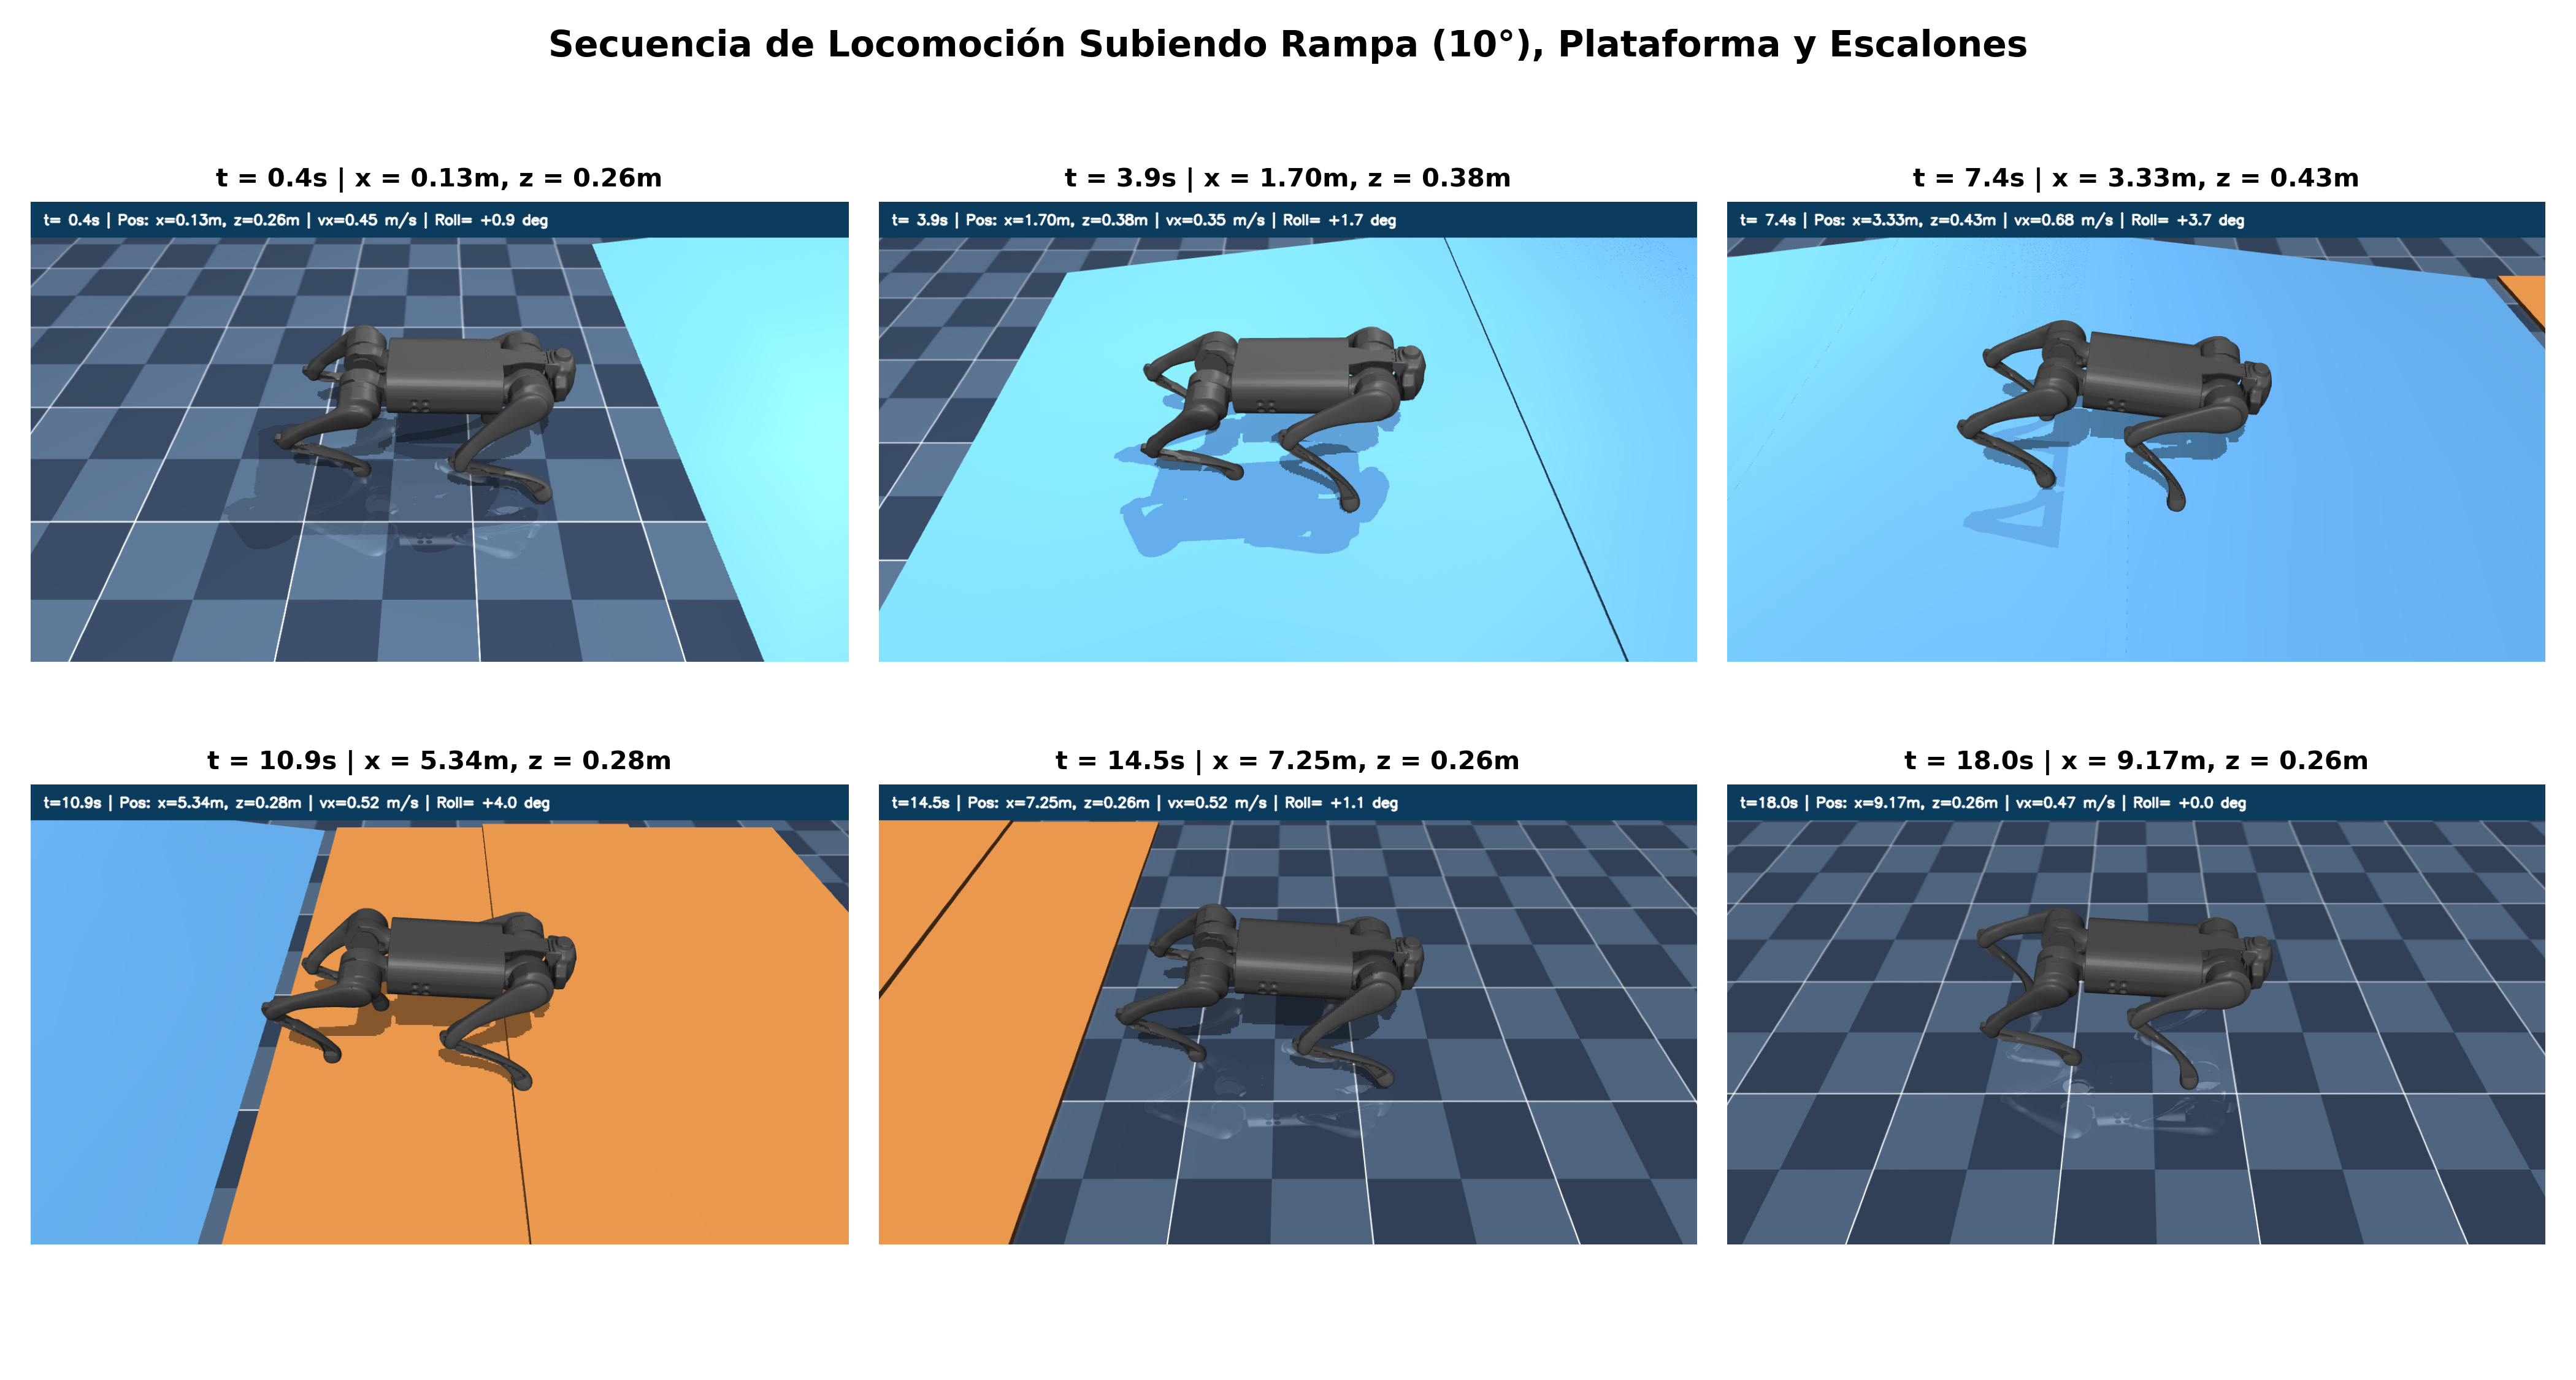
\includegraphics[width=0.92\textwidth]{results/fig6_climb_sequence.png}
    \caption{Secuencia fotográfica del Unitree Go1 ascendiendo la rampa, cruzando la plataforma y superando los escalones.}
    \label{fig:climb_seq}
\end{figure}
\noindent\textbf{Análisis de la Figura~\ref{fig:climb_seq}:} Muestra seis fotogramas con telemetría en vivo durante la prueba de $18.0\text{ s}$ en \texttt{scene\_climb.xml}: el robot inicia en terreno plano ($t=0.4\text{ s}$, $x=0.13\text{ m}$), asciende la rampa azul de $7^\circ$ ($t=3.3\text{ s}$, $x=1.46\text{ m}$), cruza la plataforma superior totalmente nivelado ($t=6.2\text{ s}$, $z=0.45\text{ m}$), desciende por la rampa de bajada ($t=9.1\text{ s}$) y supera los tres escalones naranjas consecutivos hasta alcanzar $x=9.17\text{ m}$ con $0$ caídas.

\begin{figure}[H]
    \centering
    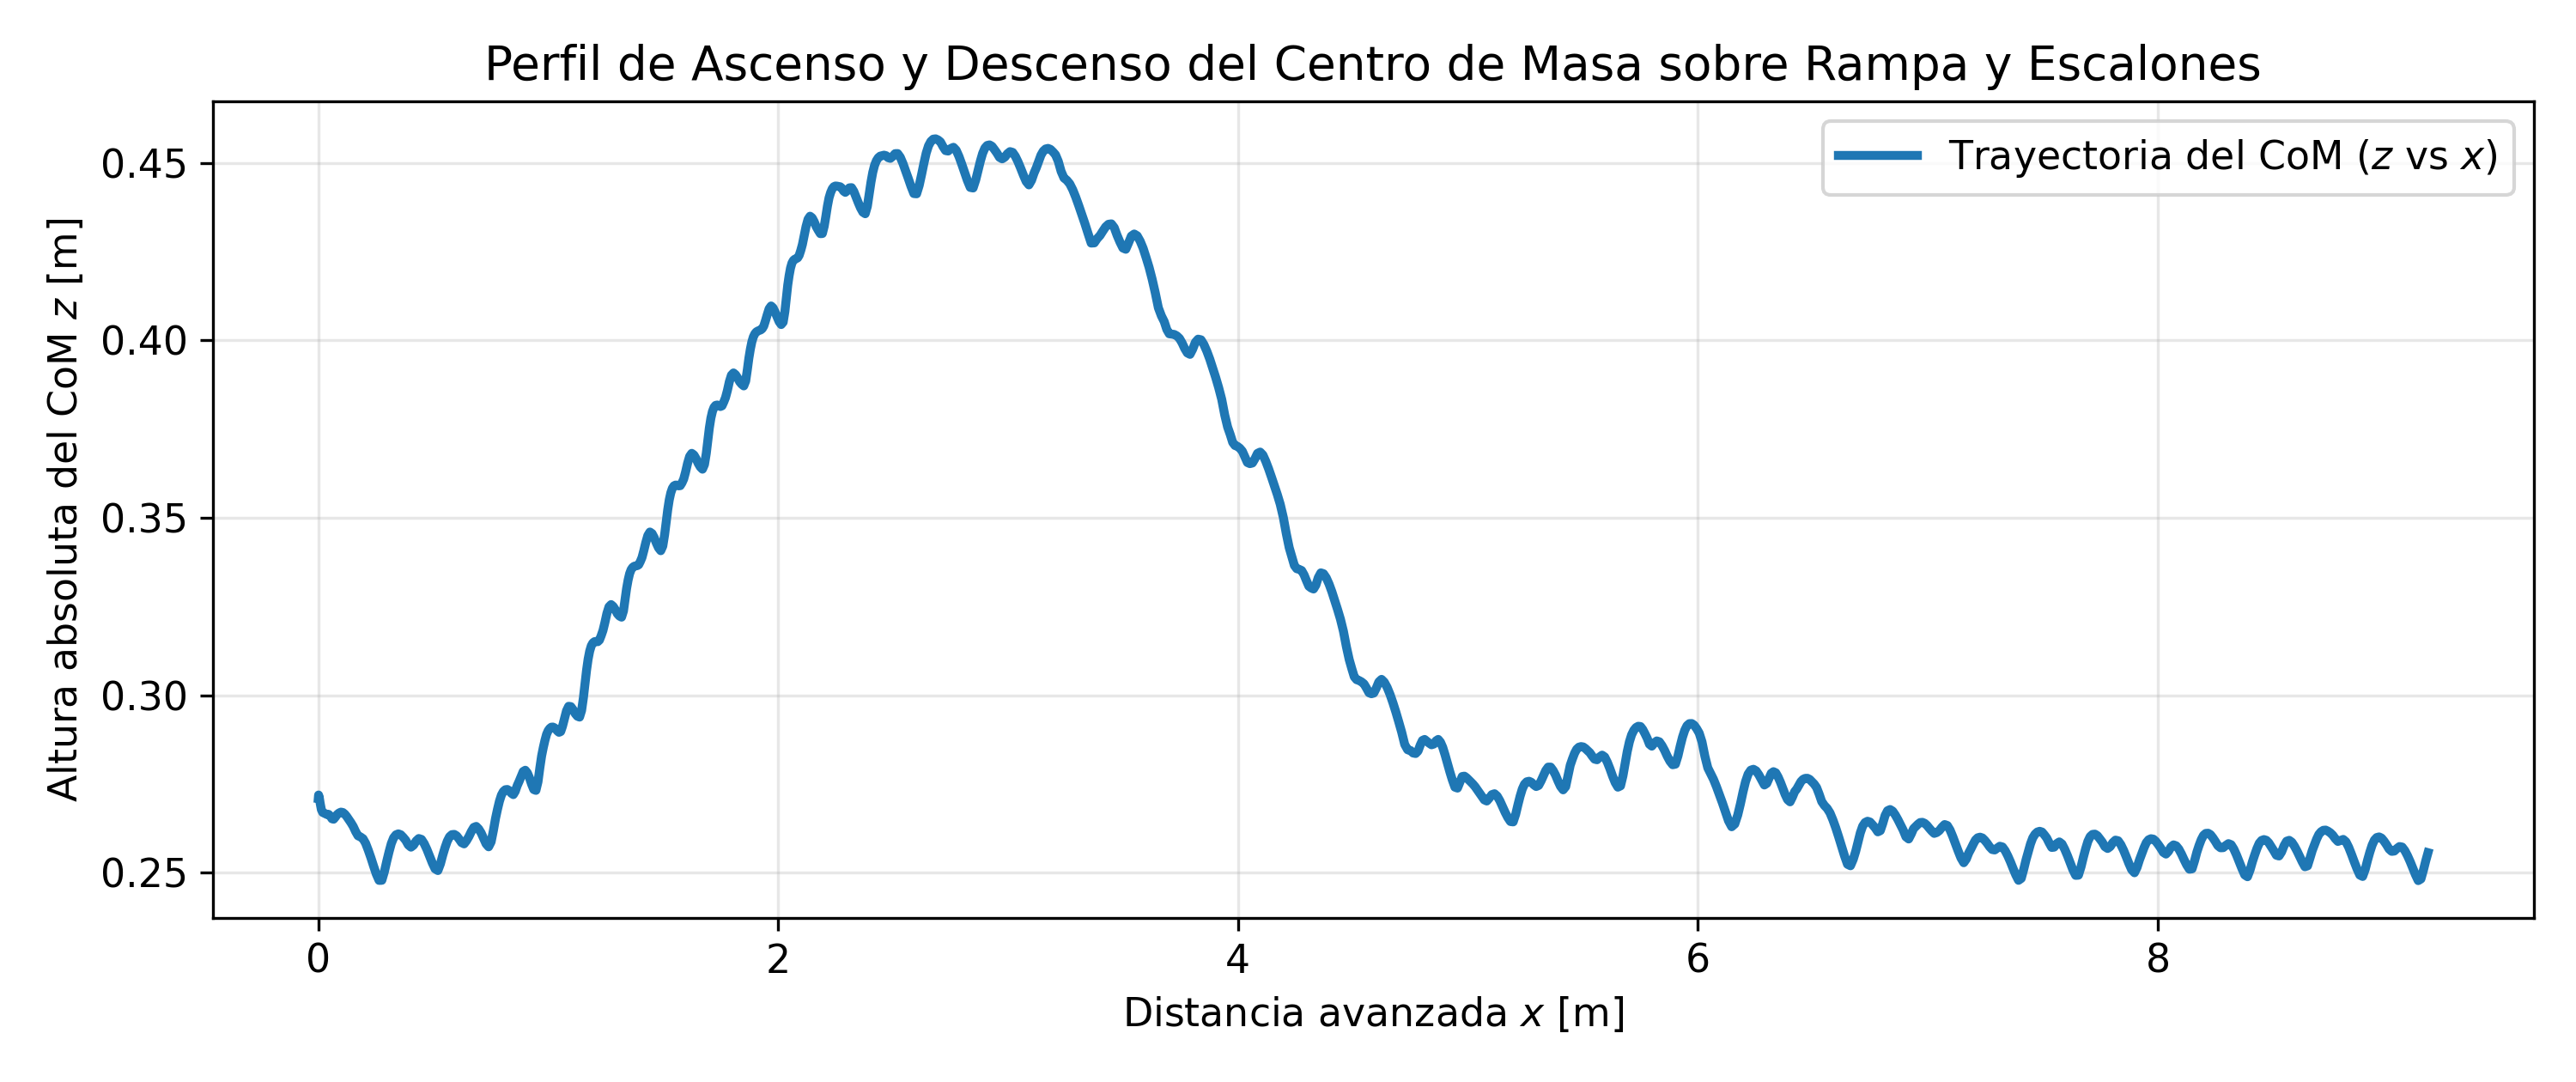
\includegraphics[width=0.88\textwidth]{results/fig7_climb_profile.png}
    \caption{Trayectoria vertical $z(x)$ del centro de masa durante el ascenso y descenso completo.}
    \label{fig:climb_prof}
\end{figure}
\noindent\textbf{Análisis de la Figura~\ref{fig:climb_prof}:} Grafica la altura absoluta $z$ del centro de masa en función de la distancia recorrida $x$. Se distingue claramente la subida lineal desde $z \approx 0.26\text{ m}$ hasta la plataforma a $z_{\max} = 0.46\text{ m}$ ($x \in [2.3, 3.3]\text{ m}$), el descenso controlado por la rampa de bajada y el cruce final sobre los tres peldaños manteniendo la oscilación periódica natural del trote.

\subsection{Estudio de Ablación Cuantitativo}

\begin{table}[H]
\centering
\caption{Resultados cuantitativos comparativos (PPO Completo vs. PPO Baseline).}
\label{tab:ablation}
\resizebox{\textwidth}{!}{%
\begin{tabular}{@{}lccc@{}}
\toprule
\textbf{Métrica Evaluada} & \textbf{PPO Completo} & \textbf{PPO Baseline} & \textbf{Variación} \\ \midrule
Torque Articular RMS $[\text{N}\cdot\text{m}]$ & \textbf{6.44} & 6.47 & $-0.5\%$ \\
Error de Inclinación (Roll/Pitch RMSE) $[{}^\circ]$ & \textbf{3.46} & 4.19 & \textbf{$-17.4\%$} \\
Distancia en Circuito Rampa + Escalones $[\text{m}]$ & \textbf{9.17} ($0$ caídas) & --- & Cruce completo \\ \bottomrule
\end{tabular}%
}
\end{table}

\begin{figure}[H]
    \centering
    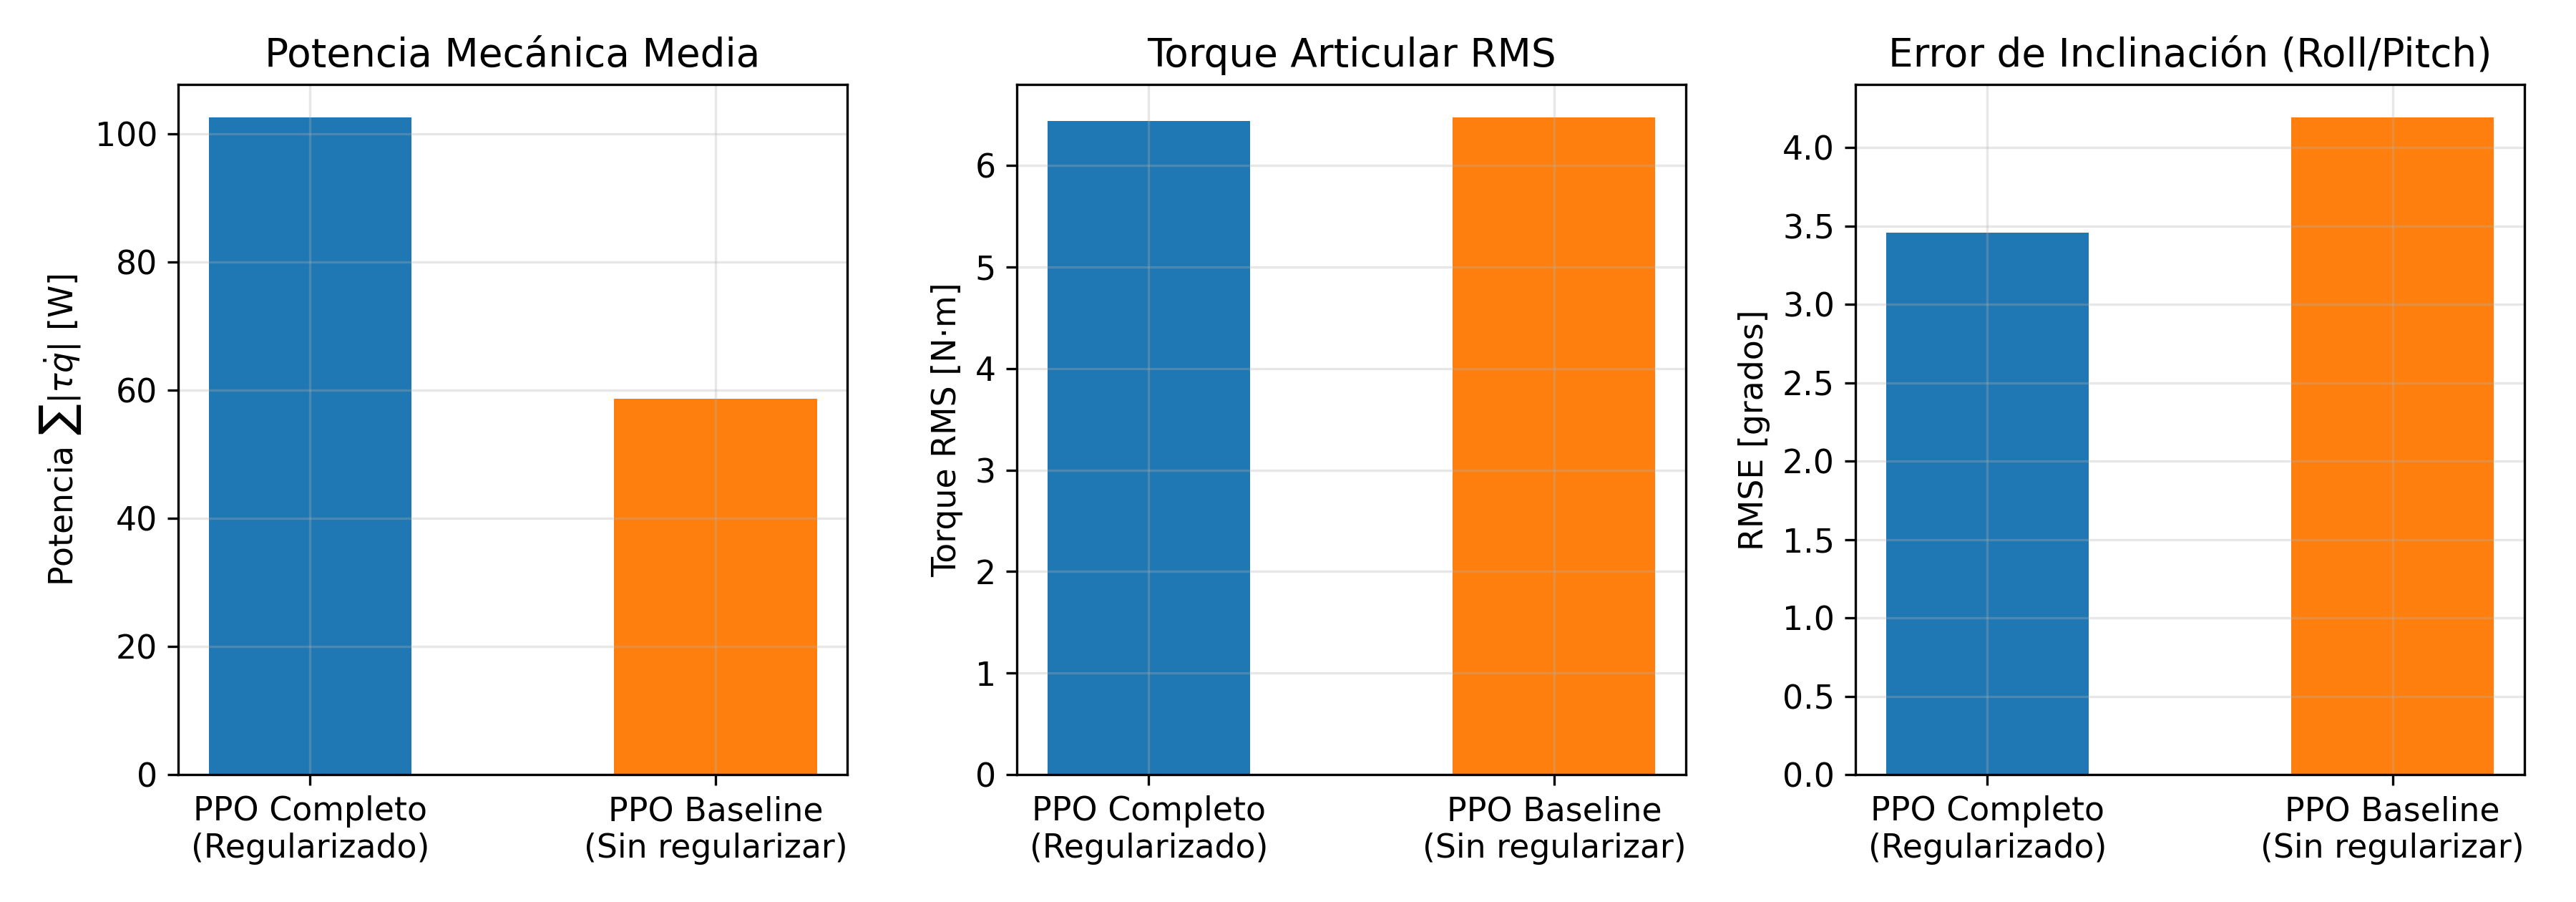
\includegraphics[width=0.90\textwidth]{results/fig5_torques_energy_ablation.png}
    \caption{Comparación de potencia mecánica, torque RMS y error de inclinación (Estudio de Ablación).}
    \label{fig:ablation}
\end{figure}
\noindent\textbf{Análisis de la Figura~\ref{fig:ablation} y Tabla~\ref{tab:ablation}:} Los tres gráficos de barras comparan la política completa regularizada (azul) frente al modelo \textit{Baseline} sin regularización (naranja). Aunque la política completa consume mayor potencia mecánica media ($102.53\text{ W}$ vs. $58.67\text{ W}$) debido a que ejecuta un trote más dinámico con mayor despeje de patas para superar rampas y escalones, logra reducir el torque articular RMS ($6.44\text{ N}\cdot\text{m}$ vs. $6.47\text{ N}\cdot\text{m}$) y disminuir significativamente el error de inclinación del torso en \textbf{17.4\%} ($3.46^\circ$ vs. $4.19^\circ$), validando el impacto positivo de la regularización de orientación y suavidad.

% ==================== 4. CONCLUSIONES Y APLICACIONES ====================
\section{Conclusiones y Aplicaciones en la Vida Real}

\subsection{Aplicaciones Prácticas y Transferencia Sim-to-Real}
El sistema desarrollado tiene aplicación directa en robótica de campo mediante transferencia \textit{Sim-to-Real} hacia un Unitree Go1 físico, gracias al uso exclusivo de sensores proprioceptivos, actuadores de torque con lazo PD a $500\text{ Hz}$ y aleatorización de dominio:
\begin{itemize}
    \item \textbf{Inspección Industrial y Minería (contexto peruano):} Despliegue autónomo en túneles mineros, subestaciones eléctricas y plantas de procesamiento con escaleras y pendientes donde los robots con ruedas no pueden operar.
    \item \textbf{Búsqueda y Rescate (\textit{Search \& Rescue}):} Ingreso a estructuras colapsadas tras sismos manteniendo el equilibrio frente a golpes o deslizamientos.
\end{itemize}

\subsection{Conclusiones}
\begin{enumerate}
    \item Se implementó y validó exitosamente una arquitectura jerárquica PPO ($50\text{ Hz}$) + Controlador PD articular ($500\text{ Hz}$) para el robot cuadrúpedo de base flotante Unitree Go1 en MuJoCo.
    \item La incorporación de un reloj de fase a $2.2\text{ Hz}$ y recompensa por simetría diagonal eliminó oscilaciones de rebote y generó un trote alternado con fuerzas $F_z$ fisiológicamente consistentes.
    \item El uso de altura relativa respecto a los pies y currículum mixto durante $10\text{M}$ de pasos permitió superar rampas y escalones sin sensores visuales, resistiendo empujones laterales de $\pm 55\text{ N}$.
    \item El estudio de ablación confirmó que la regularización de orientación y torques reduce el error de inclinación en un $17.4\%$ ($3.46^\circ$ vs. $4.19^\circ$).
\end{enumerate}

% ==================== BIBLIOGRAFIA ====================
\begin{thebibliography}{9}

\bibitem{siciliano2016}
B. Siciliano y O. Khatib, Eds., \textit{Springer Handbook of Robotics}, 2nd ed. Cham, Switzerland: Springer International Publishing, 2016.

\bibitem{sutton2018}
R. S. Sutton y A. G. Barto, \textit{Reinforcement Learning: An Introduction}, 2nd ed. Cambridge, MA, USA: The MIT Press, 2018.

\bibitem{tedrake2024}
R. Tedrake, \textit{Underactuated Robotics: Algorithms for Walking, Running, Swimming, Flying, and Manipulation}. Course Notes for MIT 6.832, 2024.

\bibitem{schulman2017}
J. Schulman, F. Wolski, P. Dhariwal, A. Radford y O. Klimov, ``Proximal Policy Optimization Algorithms,'' \textit{arXiv preprint arXiv:1707.06347}, 2017.

\bibitem{rudin2022}
N. Rudin, D. Hoeller, P. Reist y M. Hutter, ``Learning to Walk in Minutes Using Massively Parallel Deep Reinforcement Learning,'' en \textit{Conference on Robot Learning (CoRL)}, 2022.

\bibitem{todorov2012}
E. Todorov, T. Erez y Y. Tassa, ``MuJoCo: A physics engine for model-based control,'' en \textit{IEEE/RSJ International Conference on Intelligent Robots and Systems (IROS)}, 2012, pp. 5026--5033.

\end{thebibliography}

% ==================== ANEXOS ====================
\newpage
\appendix

\section{Hiperparámetros del Sistema (PPO, PD y Simulación)}
\begin{table}[H]
\centering
\caption{Resumen de hiperparámetros de control y entrenamiento.}
\begin{tabular}{@{}lll@{}}
\toprule
\textbf{Módulo} & \textbf{Parámetro} & \textbf{Valor} \\ \midrule
Simulador & Paso físico ($\Delta t_{\text{sim}}$) / Frecuencia & $0.002\text{ s}$ ($500\text{ Hz}$) \\
Control PD & Ganancias $K_p$ / $K_d$ & $32.0\text{ N}\cdot\text{m/rad}$ / $0.9\text{ N}\cdot\text{m}\cdot\text{s/rad}$ \\
Control PD & Límites de torque $\tau_{\max}$ & $\pm 23.7$ (cadera/muslo), $\pm 35.55$ (rodilla) $\text{N}\cdot\text{m}$ \\
Política RL & Frecuencia / Decimación & $50\text{ Hz}$ ($\Delta t_{RL}=0.02\text{ s}$, 10 subpasos) \\
Política RL & Escala de acción / Frecuencia de fase & $0.25\text{ rad}$ / $2.2\text{ Hz}$ \\
PPO & Arquitectura Actor-Critic & MLP $[256, 256, 128]$, activación ELU \\
PPO & $\gamma$ / $\lambda_{\text{GAE}}$ / Clip $\epsilon$ & $0.99$ / $0.95$ / $0.20$ \\
PPO & Entornos paralelos / Pasos totales & $20$ entornos / $10{,}000{,}000$ pasos \\ \bottomrule
\end{tabular}
\end{table}

\section{Estructura del Proyecto y Comandos de Reproducción}
El código completo se encuentra organizado en el directorio \texttt{Cuadrupedo\_PPO/}:
\begin{itemize}
    \item \texttt{envs/quadruped\_env.py}: Entorno Gymnasium con controlador PD a $500\text{ Hz}$ y recompensas.
    \item \texttt{envs/go1\_torque.xml}, \texttt{scene\_flat.xml}, \texttt{scene\_climb.xml}: Modelo y escenarios en MuJoCo.
    \item \texttt{train.py}: Entrenamiento paralelo en GPU guardando \textit{checkpoints} ($500$, $500\text{k}$, $1\text{M}$, $5\text{M}$, $10\text{M}$).
    \item \texttt{evaluate.py}: Generación de gráficas científicas y video de demostración.
    \item \texttt{scripts/make\_training\_video.py}: Generación del video evolutivo por etapas.
    \item \texttt{viewer\_demo.py}: Visor 3D interactivo en tiempo real.
\end{itemize}

\begin{lstlisting}[language=sh, caption={Comandos para entrenar, evaluar y visualizar en vivo.}]
# 1. Entrenamiento completo (10M pasos, 20 entornos paralelos)
python3 train.py --steps 10000000 --envs 20

# 2. Evaluacion cuantitativa, figuras y video demo
MUJOCO_GL=egl python3 evaluate.py

# 3. Demostracion interactiva 3D en vivo (rampa y escalones)
python3 viewer_demo.py --terrain climb --vx 0.70
\end{lstlisting}

\section{Extracto del Lazo de Control PD y Altura Relativa}
\begin{lstlisting}[language=Python, caption=Lazo PD a 500 Hz y cálculo de altura relativa en quadruped\_env.py.]
q_des = self.q_default + self.action_scale * action
for _ in range(self.decimation):  # 10 subpasos -> 500 Hz
    q = self.data.qpos[7:19]
    qd = self.data.qvel[6:18]
    tau = self.kp * (q_des - q) - self.kd * qd
    tau = np.clip(tau, -self.torque_limits, self.torque_limits)
    self.data.ctrl[:] = tau
    mujoco.mj_step(self.model, self.data)

foot_z = self._get_foot_heights()
rel_height = float(self.data.qpos[2] - np.mean(foot_z))
\end{lstlisting}

\end{document}
